\documentclass[1p]{elsarticle_modified}
%\bibliographystyle{elsarticle-num}

%\usepackage[colorlinks]{hyperref}
%\usepackage{abbrmath_seonhwa} %\Abb, \Ascr, \Acal ,\Abf, \Afrak
\usepackage{amsfonts}
\usepackage{amssymb}
\usepackage{amsmath}
\usepackage{amsthm}
\usepackage{scalefnt}
\usepackage{amsbsy}
\usepackage{kotex}
\usepackage{caption}
\usepackage{subfig}
\usepackage{color}
\usepackage{graphicx}
\usepackage{xcolor} %% white, black, red, green, blue, cyan, magenta, yellow
\usepackage{float}
\usepackage{setspace}
\usepackage{hyperref}

\usepackage{tikz}
\usetikzlibrary{arrows}

\usepackage{multirow}
\usepackage{array} % fixed length table
\usepackage{hhline}

%%%%%%%%%%%%%%%%%%%%%
\makeatletter
\renewcommand*\env@matrix[1][\arraystretch]{%
	\edef\arraystretch{#1}%
	\hskip -\arraycolsep
	\let\@ifnextchar\new@ifnextchar
	\array{*\c@MaxMatrixCols c}}
\makeatother %https://tex.stackexchange.com/questions/14071/how-can-i-increase-the-line-spacing-in-a-matrix
%%%%%%%%%%%%%%%

\usepackage[normalem]{ulem}

\newcommand{\msout}[1]{\ifmmode\text{\sout{\ensuremath{#1}}}\else\sout{#1}\fi}
%SOURCE: \msout is \stkout macro in https://tex.stackexchange.com/questions/20609/strikeout-in-math-mode

\newcommand{\cancel}[1]{
	\ifmmode
	{\color{red}\msout{#1}}
	\else
	{\color{red}\sout{#1}}
	\fi
}

\newcommand{\add}[1]{
	{\color{blue}\uwave{#1}}
}

\newcommand{\replace}[2]{
	\ifmmode
	{\color{red}\msout{#1}}{\color{blue}\uwave{#2}}
	\else
	{\color{red}\sout{#1}}{\color{blue}\uwave{#2}}
	\fi
}

\newcommand{\Sol}{\mathcal{S}} %segment
\newcommand{\D}{D} %diagram
\newcommand{\A}{\mathcal{A}} %arc


%%%%%%%%%%%%%%%%%%%%%%%%%%%%%5 test

\def\sl{\operatorname{\textup{SL}}(2,\Cbb)}
\def\psl{\operatorname{\textup{PSL}}(2,\Cbb)}
\def\quan{\mkern 1mu \triangleright \mkern 1mu}

\theoremstyle{definition}
\newtheorem{thm}{Theorem}[section]
\newtheorem{prop}[thm]{Proposition}
\newtheorem{lem}[thm]{Lemma}
\newtheorem{ques}[thm]{Question}
\newtheorem{cor}[thm]{Corollary}
\newtheorem{defn}[thm]{Definition}
\newtheorem{exam}[thm]{Example}
\newtheorem{rmk}[thm]{Remark}
\newtheorem{alg}[thm]{Algorithm}

\newcommand{\I}{\sqrt{-1}}
\begin{document}

%\begin{frontmatter}
%
%\title{Boundary parabolic representations of knots up to 8 crossings}
%
%%% Group authors per affiliation:
%\author{Yunhi Cho} 
%\address{Department of Mathematics, University of Seoul, Seoul, Korea}
%\ead{yhcho@uos.ac.kr}
%
%
%\author{Seonhwa Kim} %\fnref{s_kim}}
%\address{Center for Geometry and Physics, Institute for Basic Science, Pohang, 37673, Korea}
%\ead{ryeona17@ibs.re.kr}
%
%\author{Hyuk Kim}
%\address{Department of Mathematical Sciences, Seoul National University, Seoul 08826, Korea}
%\ead{hyukkim@snu.ac.kr}
%
%\author{Seokbeom Yoon}
%\address{Department of Mathematical Sciences, Seoul National University, Seoul, 08826,  Korea}
%\ead{sbyoon15@snu.ac.kr}
%
%\begin{abstract}
%We find all boundary parabolic representation of knots up to 8 crossings.
%
%\end{abstract}
%\begin{keyword}
%    \MSC[2010] 57M25 
%\end{keyword}
%
%\end{frontmatter}

%\linenumbers
%\tableofcontents
%
\newcommand\colored[1]{\textcolor{white}{\rule[-0.35ex]{0.8em}{1.4ex}}\kern-0.8em\color{red} #1}%
%\newcommand\colored[1]{\textcolor{white}{ #1}\kern-2.17ex	\textcolor{white}{ #1}\kern-1.81ex	\textcolor{white}{ #1}\kern-2.15ex\color{red}#1	}

{\Large $\underline{10_{56}~(K10a_{28})}$}

\setlength{\tabcolsep}{10pt}
\renewcommand{\arraystretch}{1.6}
\vspace{1cm}\begin{tabular}{m{100pt}>{\centering\arraybackslash}m{274pt}}
\multirow{5}{120pt}{
	\centering
	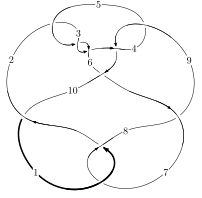
\includegraphics[width=112pt]{../../../GIT/diagram.site/Diagrams/png/140_10_56.png}\\
\ \ \ A knot diagram\footnotemark}&
\allowdisplaybreaks
\textbf{Linearized knot diagam} \\
\cline{2-2}
 &
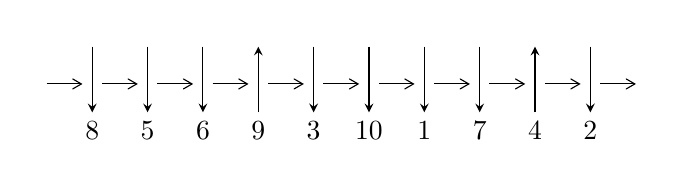
\begin{tikzpicture}[x=20pt, y=17pt]
	% nodes
	\node (C0) at (0, 0) {};
	\node (C1) at (1, 0) {};
	\node (C1U) at (1, +1) {};
	\node (C1D) at (1, -1) {8};

	\node (C2) at (2, 0) {};
	\node (C2U) at (2, +1) {};
	\node (C2D) at (2, -1) {5};

	\node (C3) at (3, 0) {};
	\node (C3U) at (3, +1) {};
	\node (C3D) at (3, -1) {6};

	\node (C4) at (4, 0) {};
	\node (C4U) at (4, +1) {};
	\node (C4D) at (4, -1) {9};

	\node (C5) at (5, 0) {};
	\node (C5U) at (5, +1) {};
	\node (C5D) at (5, -1) {3};

	\node (C6) at (6, 0) {};
	\node (C6U) at (6, +1) {};
	\node (C6D) at (6, -1) {10};

	\node (C7) at (7, 0) {};
	\node (C7U) at (7, +1) {};
	\node (C7D) at (7, -1) {1};

	\node (C8) at (8, 0) {};
	\node (C8U) at (8, +1) {};
	\node (C8D) at (8, -1) {7};

	\node (C9) at (9, 0) {};
	\node (C9U) at (9, +1) {};
	\node (C9D) at (9, -1) {4};

	\node (C10) at (10, 0) {};
	\node (C10U) at (10, +1) {};
	\node (C10D) at (10, -1) {2};
	\node (C11) at (11, 0) {};

	% arrows
	\draw[->,>={angle 60}]
	(C0) edge (C1) (C1) edge (C2) (C2) edge (C3) (C3) edge (C4) (C4) edge (C5) (C5) edge (C6) (C6) edge (C7) (C7) edge (C8) (C8) edge (C9) (C9) edge (C10) (C10) edge (C11) ;	\draw[->,>=stealth]
	(C1U) edge (C1D) (C2U) edge (C2D) (C3U) edge (C3D) (C4D) edge (C4U) (C5U) edge (C5D) (C6U) edge (C6D) (C7U) edge (C7D) (C8U) edge (C8D) (C9D) edge (C9U) (C10U) edge (C10D) ;
	\end{tikzpicture} \\
\hhline{~~} \\& 
\textbf{Solving Sequence} \\ \cline{2-2} 
 &
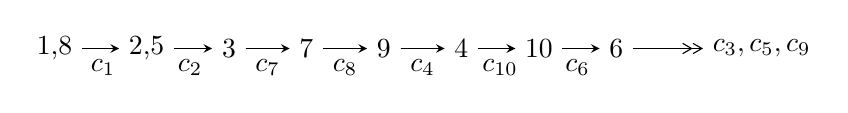
\begin{tikzpicture}[x=28pt, y=7pt]
	% node
	\node (A0) at (-1/8, 0) {1,8};
	\node (A1) at (17/16, 0) {2,5};
	\node (A2) at (17/8, 0) {3};
	\node (A3) at (25/8, 0) {7};
	\node (A4) at (33/8, 0) {9};
	\node (A5) at (41/8, 0) {4};
	\node (A6) at (49/8, 0) {10};
	\node (A7) at (57/8, 0) {6};
	\node (C1) at (1/2, -1) {$c_{1}$};
	\node (C2) at (13/8, -1) {$c_{2}$};
	\node (C3) at (21/8, -1) {$c_{7}$};
	\node (C4) at (29/8, -1) {$c_{8}$};
	\node (C5) at (37/8, -1) {$c_{4}$};
	\node (C6) at (45/8, -1) {$c_{10}$};
	\node (C7) at (53/8, -1) {$c_{6}$};
	\node (A8) at (9, 0) {$c_{3},c_{5},c_{9}$};

	% edge
	\draw[->,>=stealth]	
	(A0) edge (A1) (A1) edge (A2) (A2) edge (A3) (A3) edge (A4) (A4) edge (A5) (A5) edge (A6) (A6) edge (A7) ;
	\draw[->>,>={angle 60}]	
	(A7) edge (A8);
\end{tikzpicture} \\ 

\end{tabular} \\

\footnotetext{
The image of knot diagram is generated by the software ``\textbf{Draw programme}" developed by Andrew Bartholomew(\url{http://www.layer8.co.uk/maths/draw/index.htm\#Running-draw}), where we modified some parts for our purpose(\url{https://github.com/CATsTAILs/LinksPainter}).
}\phantom \\ \newline 
\centering \textbf{Ideals for irreducible components\footnotemark of $X_{\text{par}}$} 
 
\begin{align*}
I^u_{1}&=\langle 
2 u^{34}+4 u^{33}+\cdots+b-2,\;2 u^{34}+2 u^{33}+\cdots+a-2,\;u^{35}+2 u^{34}+\cdots-2 u-1\rangle \\
I^u_{2}&=\langle 
- u^2+b,\;a- u,\;u^3- u^2+1\rangle \\
\\
\end{align*}
\raggedright * 2 irreducible components of $\dim_{\mathbb{C}}=0$, with total 38 representations.\\
\footnotetext{All coefficients of polynomials are rational numbers. But the coefficients are sometimes approximated in decimal forms when there is not enough margin.}
\newpage
\renewcommand{\arraystretch}{1}
\centering \section*{I. $I^u_{1}= \langle 2 u^{34}+4 u^{33}+\cdots+b-2,\;2 u^{34}+2 u^{33}+\cdots+a-2,\;u^{35}+2 u^{34}+\cdots-2 u-1 \rangle$}
\flushleft \textbf{(i) Arc colorings}\\
\begin{tabular}{m{7pt} m{180pt} m{7pt} m{180pt} }
\flushright $a_{1}=$&$\begin{pmatrix}1\\0\end{pmatrix}$ \\
\flushright $a_{8}=$&$\begin{pmatrix}0\\u\end{pmatrix}$ \\
\flushright $a_{2}=$&$\begin{pmatrix}1\\u^2\end{pmatrix}$ \\
\flushright $a_{5}=$&$\begin{pmatrix}-2 u^{34}-2 u^{33}+\cdots+6 u+2\\-2 u^{34}-4 u^{33}+\cdots+2 u+2\end{pmatrix}$ \\
\flushright $a_{3}=$&$\begin{pmatrix}u^{34}+u^{33}+\cdots-4 u-1\\u^{34}+2 u^{33}+\cdots+9 u^2-1\end{pmatrix}$ \\
\flushright $a_{7}=$&$\begin{pmatrix}u\\u\end{pmatrix}$ \\
\flushright $a_{9}=$&$\begin{pmatrix}- u^3\\- u^3+u\end{pmatrix}$ \\
\flushright $a_{4}=$&$\begin{pmatrix}u^{32}-5 u^{30}+\cdots+4 u+1\\- u^{33}+5 u^{31}+\cdots-4 u^2- u\end{pmatrix}$ \\
\flushright $a_{10}=$&$\begin{pmatrix}- u^2+1\\- u^4\end{pmatrix}$ \\
\flushright $a_{6}=$&$\begin{pmatrix}- u^7+2 u^5-2 u^3+2 u\\- u^9+u^7- u^5+u\end{pmatrix}$\\&\end{tabular}
\flushleft \textbf{(ii) Obstruction class $= -1$}\\~\\
\flushleft \textbf{(iii) Cusp Shapes $= 7 u^{34}+10 u^{33}-33 u^{32}-62 u^{31}+104 u^{30}+233 u^{29}-217 u^{28}-640 u^{27}+303 u^{26}+1349 u^{25}-205 u^{24}-2310 u^{23}-276 u^{22}+3206 u^{21}+1184 u^{20}-3622 u^{19}-2289 u^{18}+3265 u^{17}+3165 u^{16}-2158 u^{15}-3352 u^{14}+824 u^{13}+2806 u^{12}+244 u^{11}-1824 u^{10}-716 u^9+828 u^8+636 u^7-230 u^6-376 u^5-32 u^4+126 u^3+61 u^2-5 u-13$}\\~\\
\newpage\renewcommand{\arraystretch}{1}
\flushleft \textbf{(iv) u-Polynomials at the component}\newline \\
\begin{tabular}{m{50pt}|m{274pt}}
Crossings & \hspace{64pt}u-Polynomials at each crossing \\
\hline $$\begin{aligned}c_{1},c_{7}\end{aligned}$$&$\begin{aligned}
&u^{35}+2 u^{34}+\cdots-2 u-1
\end{aligned}$\\
\hline $$\begin{aligned}c_{2},c_{3},c_{5}\end{aligned}$$&$\begin{aligned}
&u^{35}-4 u^{34}+\cdots+3 u-1
\end{aligned}$\\
\hline $$\begin{aligned}c_{4},c_{9}\end{aligned}$$&$\begin{aligned}
&u^{35}- u^{34}+\cdots-28 u-8
\end{aligned}$\\
\hline $$\begin{aligned}c_{6}\end{aligned}$$&$\begin{aligned}
&u^{35}-2 u^{34}+\cdots+36 u-36
\end{aligned}$\\
\hline $$\begin{aligned}c_{8},c_{10}\end{aligned}$$&$\begin{aligned}
&u^{35}+12 u^{34}+\cdots+10 u+1
\end{aligned}$\\
\hline
\end{tabular}\\~\\
\newpage\renewcommand{\arraystretch}{1}
\flushleft \textbf{(v) Riley Polynomials at the component}\newline \\
\begin{tabular}{m{50pt}|m{274pt}}
Crossings & \hspace{64pt}Riley Polynomials at each crossing \\
\hline $$\begin{aligned}c_{1},c_{7}\end{aligned}$$&$\begin{aligned}
&y^{35}-12 y^{34}+\cdots+10 y-1
\end{aligned}$\\
\hline $$\begin{aligned}c_{2},c_{3},c_{5}\end{aligned}$$&$\begin{aligned}
&y^{35}-34 y^{34}+\cdots+19 y-1
\end{aligned}$\\
\hline $$\begin{aligned}c_{4},c_{9}\end{aligned}$$&$\begin{aligned}
&y^{35}+21 y^{34}+\cdots+16 y-64
\end{aligned}$\\
\hline $$\begin{aligned}c_{6}\end{aligned}$$&$\begin{aligned}
&y^{35}-12 y^{34}+\cdots+22392 y-1296
\end{aligned}$\\
\hline $$\begin{aligned}c_{8},c_{10}\end{aligned}$$&$\begin{aligned}
&y^{35}+24 y^{34}+\cdots+10 y-1
\end{aligned}$\\
\hline
\end{tabular}\\~\\
\newpage\flushleft \textbf{(vi) Complex Volumes and Cusp Shapes}
$$\begin{array}{c|c|c}  
\text{Solutions to }I^u_{1}& \I (\text{vol} + \sqrt{-1}CS) & \text{Cusp shape}\\
 \hline 
\begin{aligned}
u &= -0.664256 + 0.761558 I \\
a &= -0.45768 - 1.47251 I \\
b &= -1.76114 - 0.11415 I\end{aligned}
 & \phantom{-}1.24148 - 2.67684 I & -4.78426 + 2.93641 I \\ \hline\begin{aligned}
u &= -0.664256 - 0.761558 I \\
a &= -0.45768 + 1.47251 I \\
b &= -1.76114 + 0.11415 I\end{aligned}
 & \phantom{-}1.24148 + 2.67684 I & -4.78426 - 2.93641 I \\ \hline\begin{aligned}
u &= -0.741471 + 0.622830 I \\
a &= -0.57819 + 1.67504 I \\
b &= \phantom{-}0.590055 + 1.240710 I\end{aligned}
 & -0.35079 + 1.76625 I & -8.73044 - 2.55261 I \\ \hline\begin{aligned}
u &= -0.741471 - 0.622830 I \\
a &= -0.57819 - 1.67504 I \\
b &= \phantom{-}0.590055 - 1.240710 I\end{aligned}
 & -0.35079 - 1.76625 I & -8.73044 + 2.55261 I \\ \hline\begin{aligned}
u &= \phantom{-}1.037620 + 0.057613 I \\
a &= \phantom{-}0.554534 - 0.308977 I \\
b &= \phantom{-}0.096321 - 0.988163 I\end{aligned}
 & -4.46867 - 2.44036 I & -13.20394 + 3.90896 I \\ \hline\begin{aligned}
u &= \phantom{-}1.037620 - 0.057613 I \\
a &= \phantom{-}0.554534 + 0.308977 I \\
b &= \phantom{-}0.096321 + 0.988163 I\end{aligned}
 & -4.46867 + 2.44036 I & -13.20394 - 3.90896 I \\ \hline\begin{aligned}
u &= -1.04680\phantom{ +0.000000I} \\
a &= \phantom{-}2.40428\phantom{ +0.000000I} \\
b &= \phantom{-}1.22975\phantom{ +0.000000I}\end{aligned}
 & -6.56245\phantom{ +0.000000I} & -13.9210\phantom{ +0.000000I} \\ \hline\begin{aligned}
u &= \phantom{-}0.647381 + 0.692758 I \\
a &= -0.044489 + 0.551561 I \\
b &= -1.82365 + 0.07795 I\end{aligned}
 & -1.45204 + 0.58793 I & -6.80279 + 0.37603 I \\ \hline\begin{aligned}
u &= \phantom{-}0.647381 - 0.692758 I \\
a &= -0.044489 - 0.551561 I \\
b &= -1.82365 - 0.07795 I\end{aligned}
 & -1.45204 - 0.58793 I & -6.80279 - 0.37603 I \\ \hline\begin{aligned}
u &= -0.636751 + 0.841462 I \\
a &= \phantom{-}0.997900 + 0.837792 I \\
b &= \phantom{-}2.05544 - 1.02610 I\end{aligned}
 & -4.54695 - 6.58963 I & -8.16646 + 3.21535 I\\
 \hline 
 \end{array}$$\newpage$$\begin{array}{c|c|c}  
\text{Solutions to }I^u_{1}& \I (\text{vol} + \sqrt{-1}CS) & \text{Cusp shape}\\
 \hline 
\begin{aligned}
u &= -0.636751 - 0.841462 I \\
a &= \phantom{-}0.997900 - 0.837792 I \\
b &= \phantom{-}2.05544 + 1.02610 I\end{aligned}
 & -4.54695 + 6.58963 I & -8.16646 - 3.21535 I \\ \hline\begin{aligned}
u &= \phantom{-}0.799224 + 0.732897 I \\
a &= -0.137052 - 0.887085 I \\
b &= \phantom{-}1.192050 - 0.720803 I\end{aligned}
 & \phantom{-}3.23509 - 1.72545 I & -0.63608 + 2.52233 I \\ \hline\begin{aligned}
u &= \phantom{-}0.799224 - 0.732897 I \\
a &= -0.137052 + 0.887085 I \\
b &= \phantom{-}1.192050 + 0.720803 I\end{aligned}
 & \phantom{-}3.23509 + 1.72545 I & -0.63608 - 2.52233 I \\ \hline\begin{aligned}
u &= \phantom{-}1.119540 + 0.118261 I \\
a &= -1.43525 + 0.93911 I \\
b &= -0.508472 + 1.022410 I\end{aligned}
 & -11.18060 - 5.92010 I & -14.7078 + 4.1258 I \\ \hline\begin{aligned}
u &= \phantom{-}1.119540 - 0.118261 I \\
a &= -1.43525 - 0.93911 I \\
b &= -0.508472 - 1.022410 I\end{aligned}
 & -11.18060 + 5.92010 I & -14.7078 - 4.1258 I \\ \hline\begin{aligned}
u &= -0.967598 + 0.636531 I \\
a &= -0.986041 - 0.154167 I \\
b &= -1.50085 + 0.53336 I\end{aligned}
 & -1.09066 + 3.19486 I & -9.71319 - 2.77080 I \\ \hline\begin{aligned}
u &= -0.967598 - 0.636531 I \\
a &= -0.986041 + 0.154167 I \\
b &= -1.50085 - 0.53336 I\end{aligned}
 & -1.09066 - 3.19486 I & -9.71319 + 2.77080 I \\ \hline\begin{aligned}
u &= \phantom{-}0.923611 + 0.710370 I \\
a &= -0.706663 + 0.972785 I \\
b &= -1.261460 - 0.179818 I\end{aligned}
 & \phantom{-}2.85420 - 3.77887 I & -1.29814 + 3.89618 I \\ \hline\begin{aligned}
u &= \phantom{-}0.923611 - 0.710370 I \\
a &= -0.706663 - 0.972785 I \\
b &= -1.261460 + 0.179818 I\end{aligned}
 & \phantom{-}2.85420 + 3.77887 I & -1.29814 - 3.89618 I \\ \hline\begin{aligned}
u &= -1.044390 + 0.520208 I \\
a &= -0.308880 - 1.070380 I \\
b &= \phantom{-}0.105718 - 0.418991 I\end{aligned}
 & -8.72011 + 1.04091 I & -12.84142 - 2.04561 I\\
 \hline 
 \end{array}$$\newpage$$\begin{array}{c|c|c}  
\text{Solutions to }I^u_{1}& \I (\text{vol} + \sqrt{-1}CS) & \text{Cusp shape}\\
 \hline 
\begin{aligned}
u &= -1.044390 - 0.520208 I \\
a &= -0.308880 + 1.070380 I \\
b &= \phantom{-}0.105718 + 0.418991 I\end{aligned}
 & -8.72011 - 1.04091 I & -12.84142 + 2.04561 I \\ \hline\begin{aligned}
u &= -0.832533\phantom{ +0.000000I} \\
a &= -0.863173\phantom{ +0.000000I} \\
b &= -0.390504\phantom{ +0.000000I}\end{aligned}
 & -1.36456\phantom{ +0.000000I} & -6.49720\phantom{ +0.000000I} \\ \hline\begin{aligned}
u &= \phantom{-}0.999651 + 0.662016 I \\
a &= \phantom{-}0.70686 - 2.15648 I \\
b &= \phantom{-}1.84700 - 0.41941 I\end{aligned}
 & -2.49390 - 5.84473 I & -8.96835 + 4.95079 I \\ \hline\begin{aligned}
u &= \phantom{-}0.999651 - 0.662016 I \\
a &= \phantom{-}0.70686 + 2.15648 I \\
b &= \phantom{-}1.84700 + 0.41941 I\end{aligned}
 & -2.49390 + 5.84473 I & -8.96835 - 4.95079 I \\ \hline\begin{aligned}
u &= \phantom{-}0.886910 + 0.817524 I \\
a &= \phantom{-}1.29729 + 0.86025 I \\
b &= \phantom{-}0.19926 + 2.00598 I\end{aligned}
 & \phantom{-}0.09589 - 3.04539 I & -10.49856 + 3.07346 I \\ \hline\begin{aligned}
u &= \phantom{-}0.886910 - 0.817524 I \\
a &= \phantom{-}1.29729 - 0.86025 I \\
b &= \phantom{-}0.19926 - 2.00598 I\end{aligned}
 & \phantom{-}0.09589 + 3.04539 I & -10.49856 - 3.07346 I \\ \hline\begin{aligned}
u &= -0.280203 + 0.733036 I \\
a &= \phantom{-}0.964828 - 0.842495 I \\
b &= \phantom{-}0.673575 - 0.185802 I\end{aligned}
 & -6.48734 + 3.48149 I & -9.01514 - 3.12997 I \\ \hline\begin{aligned}
u &= -0.280203 - 0.733036 I \\
a &= \phantom{-}0.964828 + 0.842495 I \\
b &= \phantom{-}0.673575 + 0.185802 I\end{aligned}
 & -6.48734 - 3.48149 I & -9.01514 + 3.12997 I \\ \hline\begin{aligned}
u &= -1.007860 + 0.690657 I \\
a &= \phantom{-}0.76872 + 1.59182 I \\
b &= \phantom{-}2.25197 + 0.62559 I\end{aligned}
 & \phantom{-}0.21056 + 8.20034 I & -6.93623 - 7.67757 I \\ \hline\begin{aligned}
u &= -1.007860 - 0.690657 I \\
a &= \phantom{-}0.76872 - 1.59182 I \\
b &= \phantom{-}2.25197 - 0.62559 I\end{aligned}
 & \phantom{-}0.21056 - 8.20034 I & -6.93623 + 7.67757 I\\
 \hline 
 \end{array}$$\newpage$$\begin{array}{c|c|c}  
\text{Solutions to }I^u_{1}& \I (\text{vol} + \sqrt{-1}CS) & \text{Cusp shape}\\
 \hline 
\begin{aligned}
u &= -1.045240 + 0.713362 I \\
a &= -0.03530 - 2.41846 I \\
b &= -2.14450 - 1.67720 I\end{aligned}
 & -5.78918 + 12.39880 I & -9.85333 - 7.70880 I \\ \hline\begin{aligned}
u &= -1.045240 - 0.713362 I \\
a &= -0.03530 + 2.41846 I \\
b &= -2.14450 + 1.67720 I\end{aligned}
 & -5.78918 - 12.39880 I & -9.85333 + 7.70880 I \\ \hline\begin{aligned}
u &= -0.282825 + 0.410007 I \\
a &= -0.74438 + 1.30353 I \\
b &= -0.006557 + 0.477496 I\end{aligned}
 & -0.429568 + 1.170440 I & -5.16678 - 5.64189 I \\ \hline\begin{aligned}
u &= -0.282825 - 0.410007 I \\
a &= -0.74438 - 1.30353 I \\
b &= -0.006557 - 0.477496 I\end{aligned}
 & -0.429568 - 1.170440 I & -5.16678 + 5.64189 I \\ \hline\begin{aligned}
u &= \phantom{-}0.392648\phantom{ +0.000000I} \\
a &= \phantom{-}1.74649\phantom{ +0.000000I} \\
b &= -0.848760\phantom{ +0.000000I}\end{aligned}
 & -2.15415\phantom{ +0.000000I} & -1.93570\phantom{ +0.000000I}\\
 \hline 
 \end{array}$$\newpage\newpage\renewcommand{\arraystretch}{1}
\centering \section*{II. $I^u_{2}= \langle - u^2+b,\;a- u,\;u^3- u^2+1 \rangle$}
\flushleft \textbf{(i) Arc colorings}\\
\begin{tabular}{m{7pt} m{180pt} m{7pt} m{180pt} }
\flushright $a_{1}=$&$\begin{pmatrix}1\\0\end{pmatrix}$ \\
\flushright $a_{8}=$&$\begin{pmatrix}0\\u\end{pmatrix}$ \\
\flushright $a_{2}=$&$\begin{pmatrix}1\\u^2\end{pmatrix}$ \\
\flushright $a_{5}=$&$\begin{pmatrix}u\\u^2\end{pmatrix}$ \\
\flushright $a_{3}=$&$\begin{pmatrix}u+1\\2 u^2\end{pmatrix}$ \\
\flushright $a_{7}=$&$\begin{pmatrix}u\\u\end{pmatrix}$ \\
\flushright $a_{9}=$&$\begin{pmatrix}- u^2+1\\- u^2+u+1\end{pmatrix}$ \\
\flushright $a_{4}=$&$\begin{pmatrix}u\\u^2\end{pmatrix}$ \\
\flushright $a_{10}=$&$\begin{pmatrix}- u^2+1\\- u^2+u+1\end{pmatrix}$ \\
\flushright $a_{6}=$&$\begin{pmatrix}-1\\- u^2\end{pmatrix}$\\&\end{tabular}
\flushleft \textbf{(ii) Obstruction class $= 1$}\\~\\
\flushleft \textbf{(iii) Cusp Shapes $= -2 u^2+7 u-10$}\\~\\
\newpage\renewcommand{\arraystretch}{1}
\flushleft \textbf{(iv) u-Polynomials at the component}\newline \\
\begin{tabular}{m{50pt}|m{274pt}}
Crossings & \hspace{64pt}u-Polynomials at each crossing \\
\hline $$\begin{aligned}c_{1}\end{aligned}$$&$\begin{aligned}
&u^3- u^2+1
\end{aligned}$\\
\hline $$\begin{aligned}c_{2},c_{3}\end{aligned}$$&$\begin{aligned}
&(u-1)^3
\end{aligned}$\\
\hline $$\begin{aligned}c_{4},c_{9}\end{aligned}$$&$\begin{aligned}
&u^3
\end{aligned}$\\
\hline $$\begin{aligned}c_{5}\end{aligned}$$&$\begin{aligned}
&(u+1)^3
\end{aligned}$\\
\hline $$\begin{aligned}c_{6},c_{10}\end{aligned}$$&$\begin{aligned}
&u^3- u^2+2 u-1
\end{aligned}$\\
\hline $$\begin{aligned}c_{7}\end{aligned}$$&$\begin{aligned}
&u^3+u^2-1
\end{aligned}$\\
\hline $$\begin{aligned}c_{8}\end{aligned}$$&$\begin{aligned}
&u^3+u^2+2 u+1
\end{aligned}$\\
\hline
\end{tabular}\\~\\
\newpage\renewcommand{\arraystretch}{1}
\flushleft \textbf{(v) Riley Polynomials at the component}\newline \\
\begin{tabular}{m{50pt}|m{274pt}}
Crossings & \hspace{64pt}Riley Polynomials at each crossing \\
\hline $$\begin{aligned}c_{1},c_{7}\end{aligned}$$&$\begin{aligned}
&y^3- y^2+2 y-1
\end{aligned}$\\
\hline $$\begin{aligned}c_{2},c_{3},c_{5}\end{aligned}$$&$\begin{aligned}
&(y-1)^3
\end{aligned}$\\
\hline $$\begin{aligned}c_{4},c_{9}\end{aligned}$$&$\begin{aligned}
&y^3
\end{aligned}$\\
\hline $$\begin{aligned}c_{6},c_{8},c_{10}\end{aligned}$$&$\begin{aligned}
&y^3+3 y^2+2 y-1
\end{aligned}$\\
\hline
\end{tabular}\\~\\
\newpage\flushleft \textbf{(vi) Complex Volumes and Cusp Shapes}
$$\begin{array}{c|c|c}  
\text{Solutions to }I^u_{2}& \I (\text{vol} + \sqrt{-1}CS) & \text{Cusp shape}\\
 \hline 
\begin{aligned}
u &= \phantom{-}0.877439 + 0.744862 I \\
a &= \phantom{-}0.877439 + 0.744862 I \\
b &= \phantom{-}0.215080 + 1.307140 I\end{aligned}
 & \phantom{-}1.37919 - 2.82812 I & -4.28809 + 2.59975 I \\ \hline\begin{aligned}
u &= \phantom{-}0.877439 - 0.744862 I \\
a &= \phantom{-}0.877439 - 0.744862 I \\
b &= \phantom{-}0.215080 - 1.307140 I\end{aligned}
 & \phantom{-}1.37919 + 2.82812 I & -4.28809 - 2.59975 I \\ \hline\begin{aligned}
u &= -0.754878\phantom{ +0.000000I} \\
a &= -0.754878\phantom{ +0.000000I} \\
b &= \phantom{-}0.569840\phantom{ +0.000000I}\end{aligned}
 & -2.75839\phantom{ +0.000000I} & -16.4240\phantom{ +0.000000I}\\
 \hline 
 \end{array}$$\newpage
\newpage\renewcommand{\arraystretch}{1}
\centering \section*{ III. u-Polynomials}
\begin{tabular}{m{50pt}|m{274pt}}
Crossings & \hspace{64pt}u-Polynomials at each crossing \\
\hline $$\begin{aligned}c_{1}\end{aligned}$$&$\begin{aligned}
&(u^3- u^2+1)(u^{35}+2 u^{34}+\cdots-2 u-1)
\end{aligned}$\\
\hline $$\begin{aligned}c_{2},c_{3}\end{aligned}$$&$\begin{aligned}
&((u-1)^3)(u^{35}-4 u^{34}+\cdots+3 u-1)
\end{aligned}$\\
\hline $$\begin{aligned}c_{4},c_{9}\end{aligned}$$&$\begin{aligned}
&u^3(u^{35}- u^{34}+\cdots-28 u-8)
\end{aligned}$\\
\hline $$\begin{aligned}c_{5}\end{aligned}$$&$\begin{aligned}
&((u+1)^3)(u^{35}-4 u^{34}+\cdots+3 u-1)
\end{aligned}$\\
\hline $$\begin{aligned}c_{6}\end{aligned}$$&$\begin{aligned}
&(u^3- u^2+2 u-1)(u^{35}-2 u^{34}+\cdots+36 u-36)
\end{aligned}$\\
\hline $$\begin{aligned}c_{7}\end{aligned}$$&$\begin{aligned}
&(u^3+u^2-1)(u^{35}+2 u^{34}+\cdots-2 u-1)
\end{aligned}$\\
\hline $$\begin{aligned}c_{8}\end{aligned}$$&$\begin{aligned}
&(u^3+u^2+2 u+1)(u^{35}+12 u^{34}+\cdots+10 u+1)
\end{aligned}$\\
\hline $$\begin{aligned}c_{10}\end{aligned}$$&$\begin{aligned}
&(u^3- u^2+2 u-1)(u^{35}+12 u^{34}+\cdots+10 u+1)
\end{aligned}$\\
\hline
\end{tabular}\newpage\renewcommand{\arraystretch}{1}
\centering \section*{ IV. Riley Polynomials}
\begin{tabular}{m{50pt}|m{274pt}}
Crossings & \hspace{64pt}Riley Polynomials at each crossing \\
\hline $$\begin{aligned}c_{1},c_{7}\end{aligned}$$&$\begin{aligned}
&(y^3- y^2+2 y-1)(y^{35}-12 y^{34}+\cdots+10 y-1)
\end{aligned}$\\
\hline $$\begin{aligned}c_{2},c_{3},c_{5}\end{aligned}$$&$\begin{aligned}
&((y-1)^3)(y^{35}-34 y^{34}+\cdots+19 y-1)
\end{aligned}$\\
\hline $$\begin{aligned}c_{4},c_{9}\end{aligned}$$&$\begin{aligned}
&y^3(y^{35}+21 y^{34}+\cdots+16 y-64)
\end{aligned}$\\
\hline $$\begin{aligned}c_{6}\end{aligned}$$&$\begin{aligned}
&(y^3+3 y^2+2 y-1)(y^{35}-12 y^{34}+\cdots+22392 y-1296)
\end{aligned}$\\
\hline $$\begin{aligned}c_{8},c_{10}\end{aligned}$$&$\begin{aligned}
&(y^3+3 y^2+2 y-1)(y^{35}+24 y^{34}+\cdots+10 y-1)
\end{aligned}$\\
\hline
\end{tabular}
\vskip 2pc
\end{document}